\section{Manual}
In the following section the most important functionalities of the votes system are summarized.

\subsection{Login}

The Votes login page displayed in figure \ref{F:votes_login} is the entry-point to the system. A direct login is possible by entering an already registered email address an the correct password to the account. If no account has been created the user can sign in by first select \textit{register} in the menu appearing when clicking on the top right button. If the resolution of the browser is high the menu is replaced by buttons in the black top bar. Clicking the \textit{register} button is followed by the registration page. A valid account requires a \textit{Username}, \textit{Realname}, \textit{Email} and \textit{Password}.

\begin{figure}
\centering
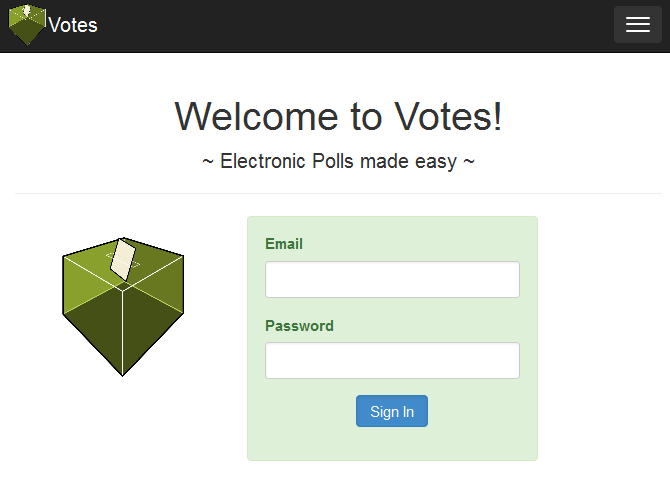
\includegraphics[width=0.4\textwidth]{png/votes_login.png}
\caption{Votes login page}
\label{F:votes_login}
\end{figure}

\subsection{Browse my Polls}
When logged in the \textit{My Polls} page, displayed in figure \ref{F:browse_my_polls}, appears. Here all polls and some poll properties can be viewed on one single page. For informations that go deeper into the Polls data the Poll has to be clicked. The table displays Poll name, state and results. The results can be viewed only when available.

\begin{figure}
\centering
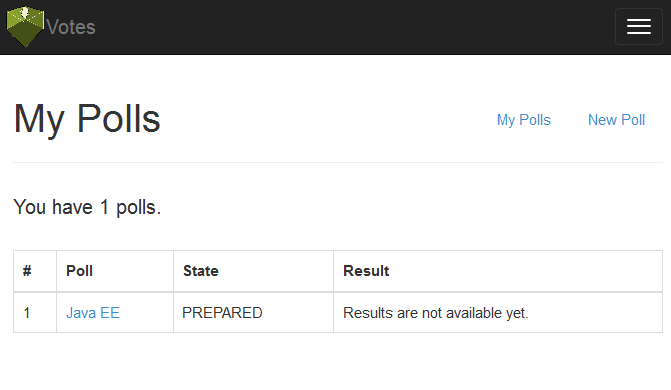
\includegraphics[width=0.4\textwidth]{png/browse_my_polls.png}
\caption{Votes login page}
\label{F:browse_my_polls}
\end{figure}



\subsection{Create and edit Polls}
